\chapter{DATA C100: Ordinary Least Squares}

\section{Multiple Linear Regression Model}
We have seen Simple Linear Regression Model, which uses one parameter for a constant term and another parameter to introduce the predictor variable. \\
The model currently has one predictor variable. \\
What if we can use more? What if we need to use more? What if our model would benefit greatly because what we attempt to predict in nature requires two or more variables for a good prediction? \\
If so, such a model would have some regression equation whose shape is to a huge degree similarly shaped as below:
\[\hat{y} = \theta_0 + \theta_1 x_1 + \theta_2 x_2 + \cdots + \theta_p x_p\]
Let us attempt to vectorize the above equation. Suppose, we rewrite the above equation as follows:
\[
    \hat{y}^{(i)} = 
    \begin{bmatrix} 1 & x_1^{(i)} & \cdots & x_p^{(i)} \end{bmatrix}
    \begin{bmatrix} \theta_0 \\ \vdots \\ \theta_p \end{bmatrix}
\]
Then, we have successfully written the above equation in a matrix-vector multiplication form. \\

Now, since there have been a lot of conventions across machine learning on how to notate vectors and features, I will be unifying my own version of conventions in this model and tailor it to the more common notations. \\
My anatomy of each term in the above row vector, $x_k^{(i)}$, is as follows:
\begin{bindenum}
    \item $x^{(i)}$ stands for the $i^{th}$ data point inside the dataset.
    \item $x_k$ stands for the $k^{th}$ feature inside the dataset.
    \item Therefore, $x_k^{(i)}$ is the $k^{th}$ feature of $i^{th}$ data point inside the dataset.
\end{bindenum}
To vectorize this operation across numerous datapoints in the dataset, we may then formulate this model in terms of matrix-vector multiplication as follows:
\[
    \begin{bmatrix} \hat{y}_1 \\ \vdots \\ \hat{y}_k \end{bmatrix} =
    \begin{bmatrix} 
        1 & x_1^{(1)} & \cdots & x_p^{(1)} \\
        \vdots & \vdots & \vdots & \vdots \\
        1 & x_1^{(k)} & \cdots & x_p^{(k)}
    \end{bmatrix}
    \begin{bmatrix} \theta_0 \\ \vdots \\ \theta_p \end{bmatrix}
\]
The column of $1$ exists for intercepts, and is important for the mathematical advantage it brings. We will discuss this later. \\
Take notes that each term can then be respectively abbreviated into what is shown below:
\[\Y = \X \theta\]
Where we specifically name the matrix $\X$ containing the datapoints as the \textbf{design matrix}.

\section{Optimization of Model: Least Squares Algorithm}

\subsection{Loss Function}
The Loss function most frequently applied for such a model has to deal with a linear algebraic property called L2 Norm:
\begin{ln-define}{L2 Norm}{}
    The L2 Norm of a vector $\vec{x} \in \R^n$ is mathematically expressed as:
    \[{||x||}_2 = \sqrt{\sum_{i = 1}^n x_i^2}\]
    which occurs to be the magnitude of such vector $\vec{x}$. \\
    We thus notate the distance of vectors $\vec{a}, \vec{b} \in \R^n$ as:
    \[{||a - b||}_2\]
\end{ln-define}
Our L2 loss function would be the distance between estimation and observed values, squared:
\[{||\Y - \hat{\Y}||}_2^2\]
Therefore yielding the empirical risk:
\[R(\theta) = \frac{1}{n} {||\Y - \X \theta||}_2^2\]

\subsection{Optimization via Geometric Interpretation}
We should first observe with our prior knowledge from EECS 16A (or alternatively MATH 54, just any college linear algebra introductory course), that since $\hat{Y}$ is a linear combination of the columns of $\X$ (as noted $\hat{Y} = \X \theta$),
\[\hat{\Y} \in span(\X) \subseteq \R^k\]
However, it is not necessary that $\Y$ belongs to the span of $\X$. Therefore, we see more clearly that our task is to minimize the distance between $\Y \notin span(\X)$ and $\hat{\Y} \in span(\X)$. \\
Let us observe a visualization from the DATA C100 Lecture Slides (since mine are underqualified and old):
\begin{ln-fig}{Geometric Image of Residual in Multiple Linear Regression}{}
    \begin{center}
        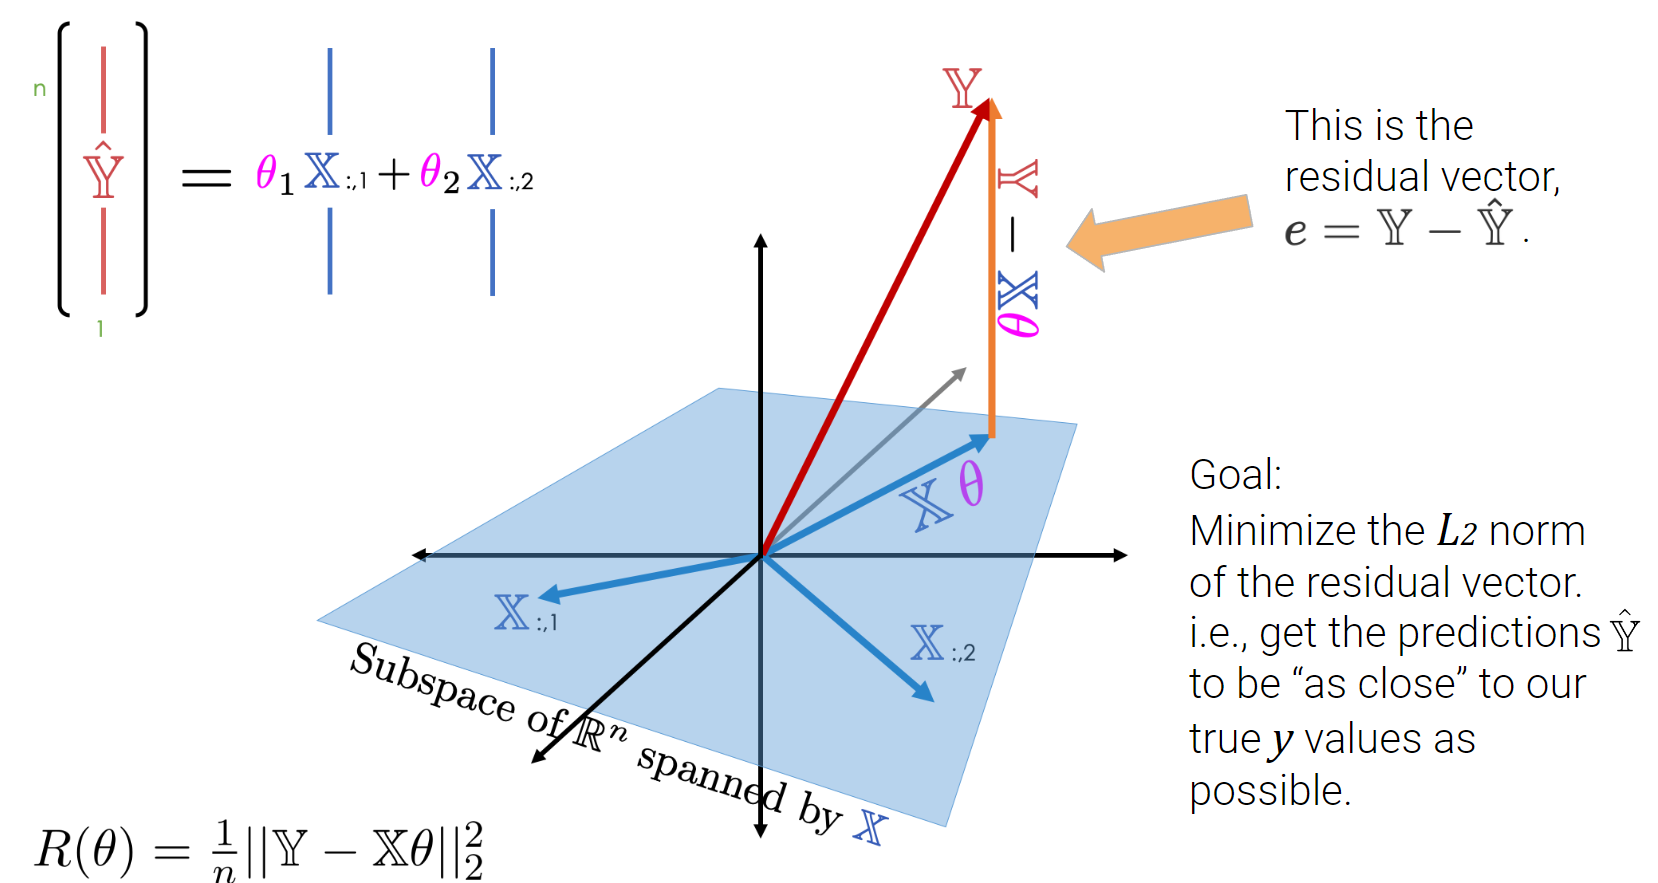
\includegraphics[scale=0.3]{figs/ln03/least-square-geometry.png}
    \end{center}
\end{ln-fig}
This residual vector is essentially the shortest possible (minimized) when it is orthogonal to $\X \theta$ (which, in a 2D view, has to do with a property of right triangles called the Pythagorean Theorem). \\
There is a better intuition than Pythagorean Theorem, which is that the vector in $span(\X)$ closest to $\Y$ must be its projection onto $span(\X)$. \\
Either way, we will be introduced to a simplified situation:
\begin{quote}
    To minimize 
    \[R(\theta) = \frac{1}{n} {||\Y - \X \theta||}_2^2\]
    We require that
    \[\X^T (\Y - \X \hat{\theta}) = 0\]
    Such that the residual $(\Y - \X \hat{\theta})$ is orthogonal to $span(\X)$.
\end{quote}
Let us review its solution from EECS 16A (or MATH 54, MATH 110):
\begin{ln-derive}{Least Squares Algorithm}{}
    \begin{align*}
        \X^T (\Y - \X \hat{\theta}) &= 0 \\
        \X^T\Y &= \X^T\X \hat{\theta} \\
        \hat{\theta} &= {(\X^T\X)}^{-1} \X^T\Y
    \end{align*}
\end{ln-derive}
Let's use calculus to see if the geometrical solution does indeed yield an optimal parameter:
\begin{ln-derive}{Least Squares Algorithm via Calculus}{}
    Remember that:
    \[
        MSE(\theta) = \frac{1}{n} \sum_{i = 1}^n {(y_i - \theta_0 - \theta_1 x_{i, 1} - \cdots - \theta_p x_{i, p})}^2
    \]
    Where, let us consider that $x_0 = 1$ exists as a part of the datapoints (row vectors), and that we have parameters from $\theta_0$ to $\theta_p$, forming a vector of $p + 1$ parameters. \\
    Then, let us differentiate such function with respect to some parameter $\theta_j$:
    \begin{align*}
        \pdv{MSE}{\theta_j}(\theta)
        &= \frac{1}{n} \sum_{i = 1}^n 2 \times -x_{i, j} \times (y_i - \theta_0 - \theta_1 x_{i, 1} - \cdots - \theta_p x_{i, p}) \\
        &= \frac{-2}{n} \sum_{i = 1}^n x_{i, j}(y_i - \theta_0 - \theta_1 x_{i, 1} - \cdots - \theta_p x_{i, p}) \\
    \end{align*}
    Which, if we optimize by setting this partial derivative to $0$, will offer us the equation that:
    \[
        \sum_{i = 1}^n x_{i, j}(y_i - \theta_0 - \theta_1 x_{i, 1} - \cdots - \theta_p x_{i, p}) = 0
    \]
    And in turn, tells that:
    \[
        \X_j^T (Y - \X^T \theta) = 0
    \]
    Therefore, differentiating the MSE loss function by some $j^{th}$ parameter provides us the normal equation by that parameter.
\end{ln-derive}
The equation above that shows the optimal parameters is known as the \textbf{Normal Equation}. \\
This normal equation would only be useful when $\X^T \X$ is invertible. Determining whether $\X^T \X$ is invertible is not as difficult as it sounds, since $N(A^T A) = N(A)$. Proof will not be showcased here. \\
Beyond the scope of DATA C100, we should also see some remedy for such situations when attempting to solve this exact optimization problem and working with a non-invertible design matrix. It is also not in the scope of this note yet.

\section{Performance Factors}
Just like in previous models, the residuals should be uncorrelated with the predicted values $\hat{y}$. \\
To determine the correlation of variables in a multivariable perspective like in Multiple Linear Regression, we work with a new coefficient:
\begin{ln-define}{Coefficient of Determination}{}
    The coefficient of determination characterizes the correlation of variables in a Multiple Linear Regression model:
    \[R^2 = \frac{\text{Variance of predicted values}}{\text{Variance of observed values}} = \frac{\sigma_{\hat{y}}^2}{\sigma_y^2}\]
\end{ln-define}
Just like the Pearson's Correlation Coefficient ($r$ in Simple Linear Regression), $R^2$ spans between $0$ and $1$ (except it is the absolute value of $r$ that spans between $0$ and $1$, not $r$ itself).
